\documentclass[aspectratio=169,12pt]{beamer}

\usetheme{Madrid}
\usecolortheme{default}
\usepackage{graphicx}
\usepackage{booktabs}
\usepackage{amsmath,amssymb}
\usepackage{tikz}
\usepackage{natbib}

% IMF-style colors
\definecolor{imfblue}{RGB}{0,51,102}
\definecolor{imfgold}{RGB}{198,146,20}
\setbeamercolor{structure}{fg=imfblue}
\setbeamercolor{title}{fg=white,bg=imfblue}
\setbeamercolor{frametitle}{fg=white,bg=imfblue}
\setbeamercolor{block title}{fg=white,bg=imfblue}
\setbeamercolor{block body}{bg=imfblue!10}

% Remove navigation symbols
\setbeamertemplate{navigation symbols}{}
\setbeamertemplate{footline}[frame number]

\title[QMIPF Julia]{Replication of the QMIPF Model in Julia}
\subtitle{Nonlinear Solution Methods for the Integrated Policy Framework}
\author{M\'aty\'as Farkas}
\institute{International Monetary Fund}
\date{\today}

\begin{document}

% Title slide
\begin{frame}
\titlepage
\end{frame}

% Outline
\begin{frame}{Outline}
\tableofcontents
\end{frame}

%=============================================================================
\section{Motivation and Objectives}
%=============================================================================

\begin{frame}{What Is This Project?}

\begin{columns}[T]
\begin{column}{0.5\textwidth}
\textbf{Original QMIPF} \citep{adrian2021quantitative}
\begin{itemize}
\item 180+ equations in Dynare/Matlab
\item First-order perturbation solution
\item Linear impulse responses
\end{itemize}

\vspace{0.5cm}
\textbf{New Julia Implementation}
\begin{itemize}
\item Full replication in MacroModelling.jl
\item 200 variables, 120 shocks, 119 parameters
\item Validated against Dynare
\end{itemize}
\end{column}

\begin{column}{0.5\textwidth}
\textbf{Why Julia?}
\begin{itemize}
\item \textcolor{imfblue}{\textbf{Stochastic Extended Path}} (SEP)
\begin{itemize}
\item Nonlinear solution with future uncertainty
\item Gauss-Hermite quadrature integration
\end{itemize}
\item \textcolor{imfblue}{\textbf{Mixed Complementarity Problems}}
\begin{itemize}
\item Occasionally binding constraints
\item ZLB, debt limits, capital controls
\end{itemize}
\item Modern, fast, open-source ecosystem
\end{itemize}
\end{column}
\end{columns}

\vspace{0.3cm}
\begin{block}{Key Message}
Julia-native QMIPF that \textbf{matches Dynare} and \textbf{goes beyond it}
\end{block}

\end{frame}

%=============================================================================
\section{Model Structure}
%=============================================================================

\begin{frame}{What Does the Model Capture?}

\begin{columns}[T]
\begin{column}{0.55\textwidth}
\textbf{Core Structure}
\begin{itemize}
\item Small open economy
\item Nominal rigidities (Calvo)
\begin{itemize}
\item Domestic prices: $\xi_p = 0.63$
\item Import prices: $\xi_m = 0.93$
\item Wages: $\xi_w = 0.81$
\end{itemize}
\item CES aggregation (domestic + imports)
\item Real UIP with risk premium
\end{itemize}

\vspace{0.3cm}
\textbf{Model Size}
\begin{itemize}
\item 200 total variables (101 auxiliary)
\item 145 state variables
\item 120 shocks
\end{itemize}
\end{column}

\begin{column}{0.45\textwidth}
\textbf{IPF Policy Tools}

\vspace{0.2cm}
\begin{enumerate}
\item \textbf{Monetary Policy}
\begin{itemize}
\item Taylor rule
\item Output gap + inflation targeting
\end{itemize}

\vspace{0.2cm}
\item \textbf{FX Intervention}
\begin{itemize}
\item $\tau_t^F$ wedge in UIP
\item Tax/subsidy on foreign borrowing
\end{itemize}

\vspace{0.2cm}
\item \textbf{Capital Flow Management}
\begin{itemize}
\item Debt limits (MCP)
\item Risk premium channel
\end{itemize}
\end{enumerate}
\end{column}
\end{columns}

\end{frame}

\begin{frame}{Key Model Equations}

\textbf{Real UIP with Endogenous Risk Premium}
\begin{equation*}
I_t (1 - \tau_t^F) = \frac{\Pi_{C,t+1}}{\Pi_{C,t+1}^*} I_t^* \frac{Q_{t+1}}{Q_t} + I_t \gamma_0 \sigma_\varepsilon^{\gamma_1} \frac{NFA_t}{\bar{Y}}
\end{equation*}

\begin{itemize}
\item LHS: Domestic return adjusted for FX intervention
\item RHS: Foreign return + expected depreciation + risk premium (Gabaix-Maggiori)
\end{itemize}

\vspace{0.3cm}
\textbf{Household Euler Equation}
\begin{equation*}
\Lambda_t = \beta \mathbb{E}_t \left[ \frac{\varsigma_{t+1}}{\varsigma_t} \frac{I_t}{\Pi_{C,t+1}} \Lambda_{t+1} \right]
\end{equation*}

\vspace{0.3cm}
\textbf{Taylor Rule}
\begin{equation*}
I_t = I_{t-1}^{\rho_i} \left( \bar{I} \left(\frac{\Pi_t^C}{\bar{\Pi}^C}\right)^{\phi_\pi} \left(\frac{Y_t}{Y_t^{pot}}\right)^{\phi_y} \right)^{1-\rho_i}
\end{equation*}

\end{frame}

%=============================================================================
\section{Validation: Julia Matches Dynare}
%=============================================================================

\begin{frame}{Three-Way Comparison: 1$\sigma$ Shocks}

\begin{columns}[T]
\begin{column}{0.4\textwidth}
\textbf{Solution Methods Compared}
\begin{enumerate}
\item \textcolor{blue}{\textbf{Dynare}} (blue solid)
\begin{itemize}
\item First-order perturbation
\item Reference implementation
\end{itemize}

\vspace{0.2cm}
\item \textcolor{green!60!black}{\textbf{Julia Deterministic SEP}} (green dashed)
\begin{itemize}
\item Order = 0
\item Perfect foresight
\end{itemize}

\vspace{0.2cm}
\item \textcolor{red}{\textbf{Julia Stochastic SEP}} (red dotted)
\begin{itemize}
\item Order = 20
\item Gauss-Hermite quadrature
\end{itemize}
\end{enumerate}
\end{column}

\begin{column}{0.6\textwidth}
\textbf{Validation Results}
\begin{itemize}
\item Perfect alignment at 1$\sigma$ shocks
\item Peak response difference: $<0.1\%$
\item All three methods yield identical IRFs
\end{itemize}

\vspace{0.3cm}
\begin{block}{Interpretation}
\begin{itemize}
\item Julia implementation validated
\item Linear approximation accurate for small shocks
\item Nonlinearities minimal at calibrated volatility
\end{itemize}
\end{block}
\end{column}
\end{columns}

\end{frame}

\begin{frame}{Productivity Shock: 1$\sigma$}
\centering
\IfFileExists{figures/QMIPF_EPS_Z_1sigma.pdf}{%
  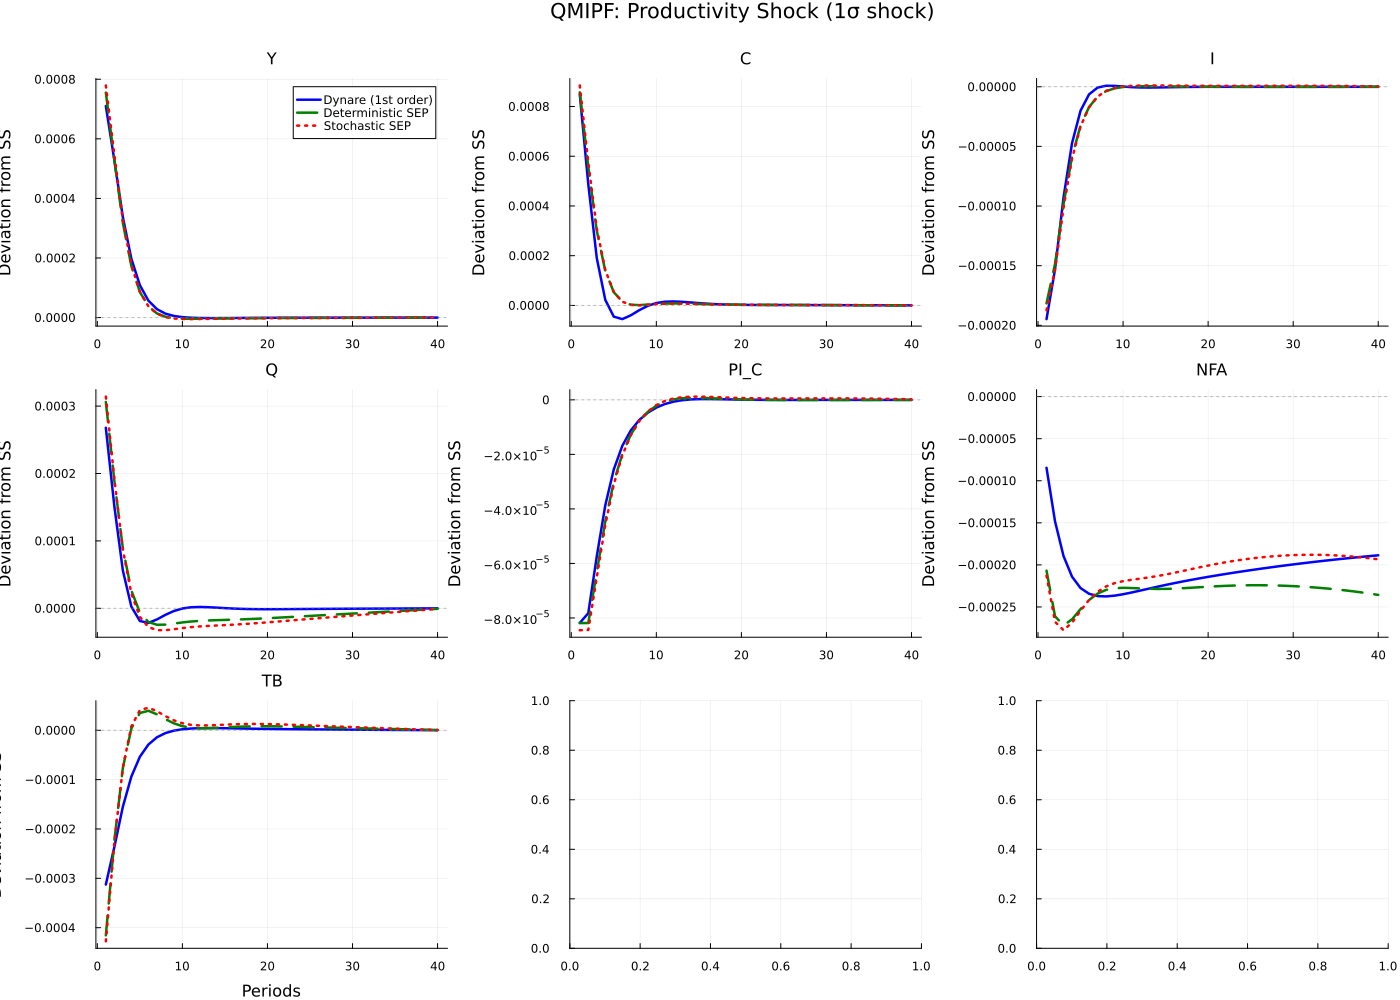
\includegraphics[width=0.6\textwidth]{figures/QMIPF_EPS_Z_1sigma.pdf}
}{%
  \fbox{\parbox{0.6\textwidth}{\centering\vspace{2cm}Figure: QMIPF\_EPS\_Z\_1sigma.pdf\vspace{2cm}}}
}
\end{frame}

\begin{frame}{Foreign Interest Rate Shock: 1$\sigma$}
\centering
\IfFileExists{figures/QMIPF_EPS_I_ST_1sigma.pdf}{%
  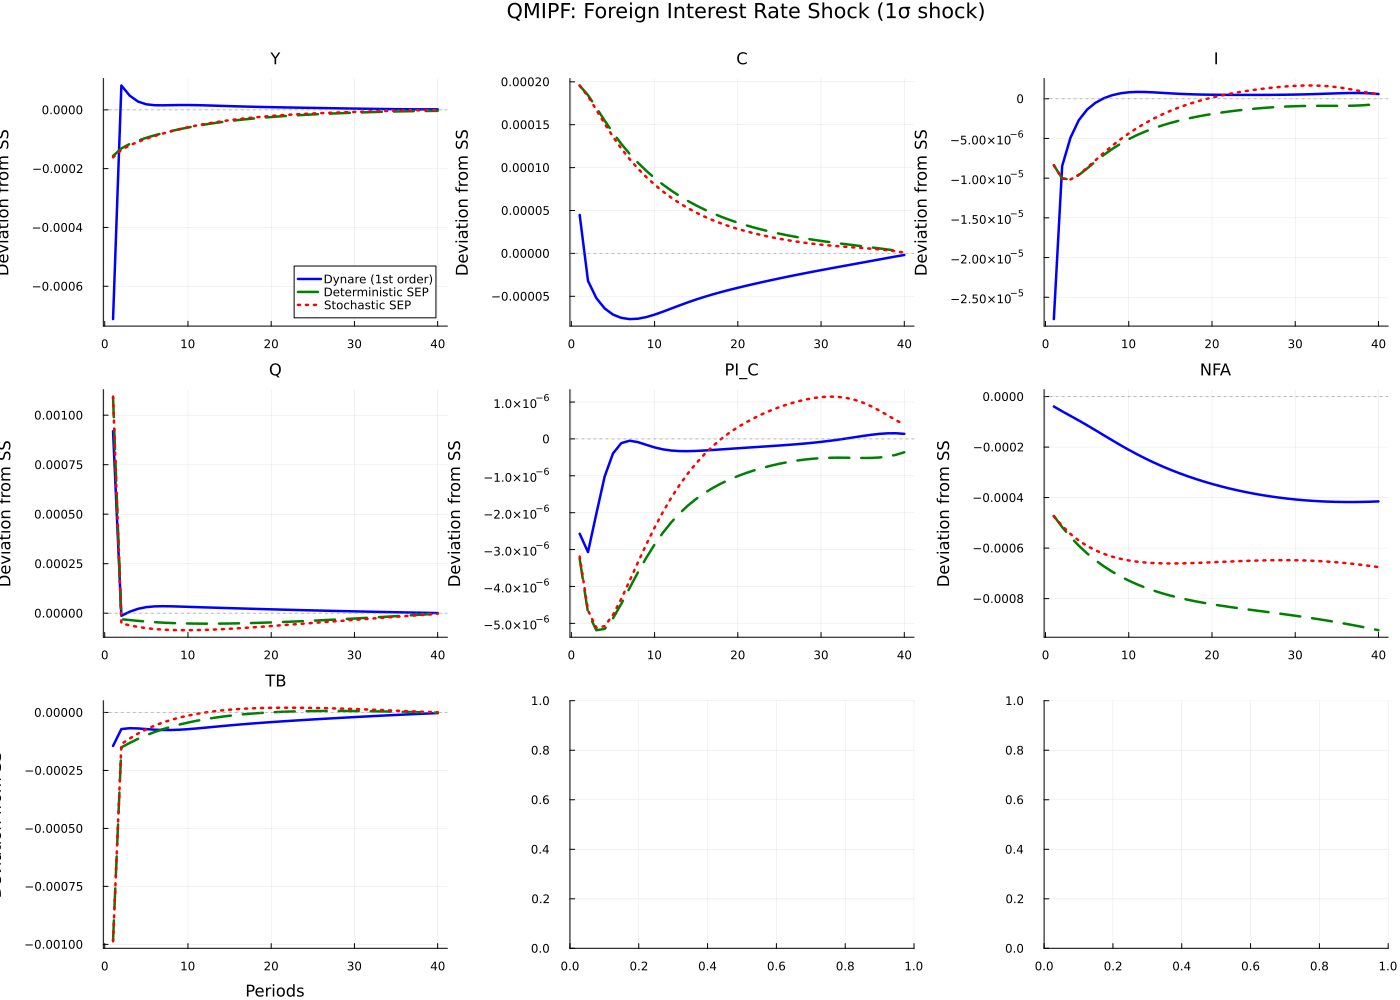
\includegraphics[width=0.6\textwidth]{figures/QMIPF_EPS_I_ST_1sigma.pdf}
}{%
  \fbox{\parbox{0.8\textwidth}{\centering\vspace{2cm}Figure: QMIPF\_EPS\_I\_ST\_1sigma.pdf\vspace{2cm}}}
}
\end{frame}

\begin{frame}{Risk Premium Shock: 1$\sigma$}
\centering
\IfFileExists{figures/QMIPF_EPS_TAU_F_1sigma.pdf}{%
  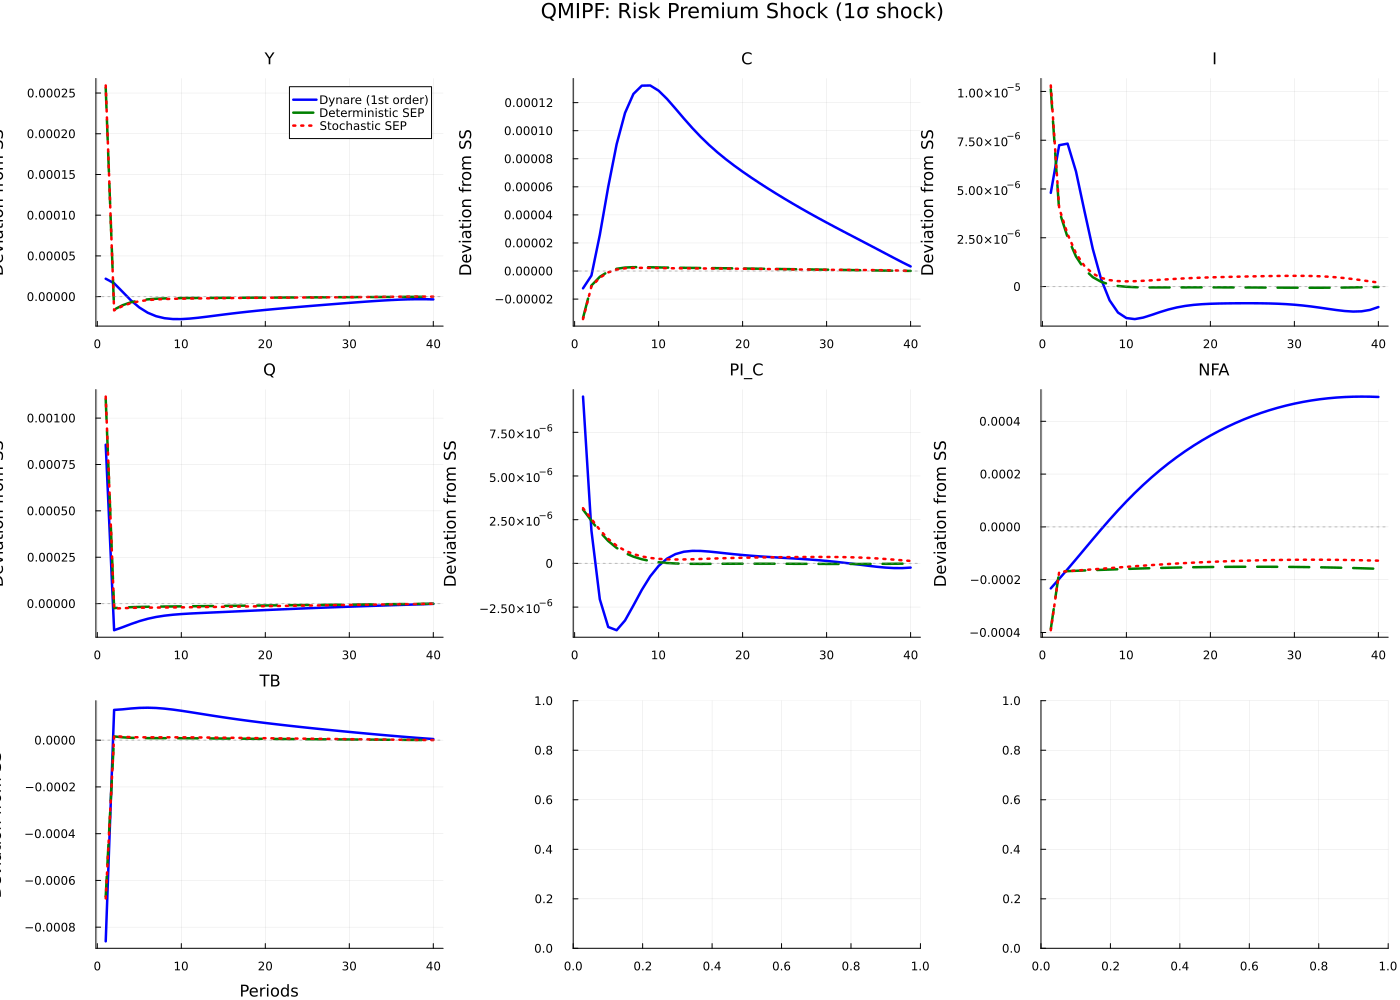
\includegraphics[width=0.6\textwidth]{figures/QMIPF_EPS_TAU_F_1sigma.pdf}
}{%
  \fbox{\parbox{0.8\textwidth}{\centering\vspace{2cm}Figure: QMIPF\_EPS\_TAU\_F\_1sigma.pdf\vspace{2cm}}}
}
\end{frame}

%=============================================================================
\section{The Novelty: Impact of Future Uncertainty}
%=============================================================================

\begin{frame}{What Stochastic SEP Captures}

\begin{columns}[T]
\begin{column}{0.5\textwidth}
\textbf{The Algorithm}
\begin{itemize}
\item Agents integrate over \textbf{future} shock realizations
\item Gauss-Hermite quadrature (3 nodes/shock)
\item Order = 20: look 20 periods ahead
\item Sparse tree for computational efficiency
\end{itemize}

\vspace{0.3cm}
\textbf{What Linear Methods Miss}
\begin{itemize}
\item Certainty equivalence assumption
\item No precautionary behavior
\item Symmetric responses to $\pm$ shocks
\end{itemize}
\end{column}

\begin{column}{0.5\textwidth}
\textbf{Key Findings at 2--3$\sigma$}

\vspace{0.2cm}
\begin{block}{Precautionary Dampening}
Stochastic SEP shows \textbf{4--9\% smaller} responses than deterministic
\end{block}

\vspace{0.2cm}
\begin{itemize}
\item Output ($Y$): $-4.8\%$
\item Consumption ($C$): $-3.6\%$
\item Investment ($I$): $-7.9\%$
\item Inflation ($\Pi^C$): $-9.2\%$
\end{itemize}

\vspace{0.2cm}
\textbf{Exception:} NFA \textit{amplified} (+0.6\%)
\begin{itemize}
\item Portfolio rebalancing under uncertainty
\end{itemize}
\end{column}
\end{columns}

\end{frame}

\begin{frame}{Productivity Shock: 2$\sigma$ and 3$\sigma$}
\begin{columns}
\begin{column}{0.5\textwidth}
\centering
\IfFileExists{figures/QMIPF_EPS_Z_2sigma.pdf}{%
  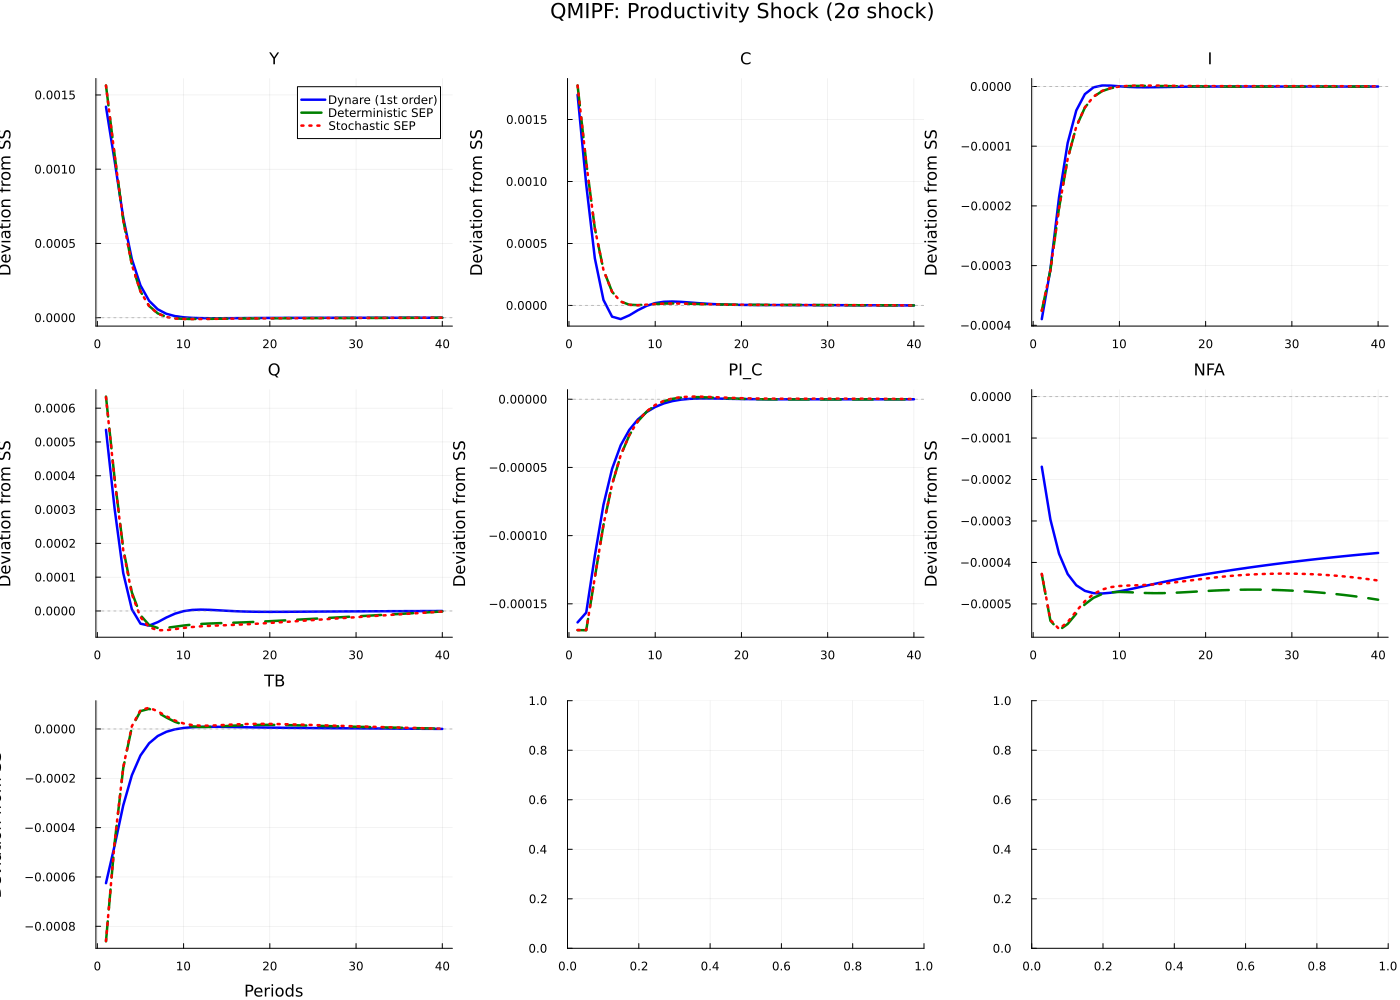
\includegraphics[width=\textwidth]{figures/QMIPF_EPS_Z_2sigma.pdf}
}{%
  \fbox{\parbox{0.9\textwidth}{\centering\vspace{1.5cm}2$\sigma$ shock\vspace{1.5cm}}}
}
\end{column}
\begin{column}{0.5\textwidth}
\centering
\IfFileExists{figures/QMIPF_EPS_Z_3sigma.pdf}{%
  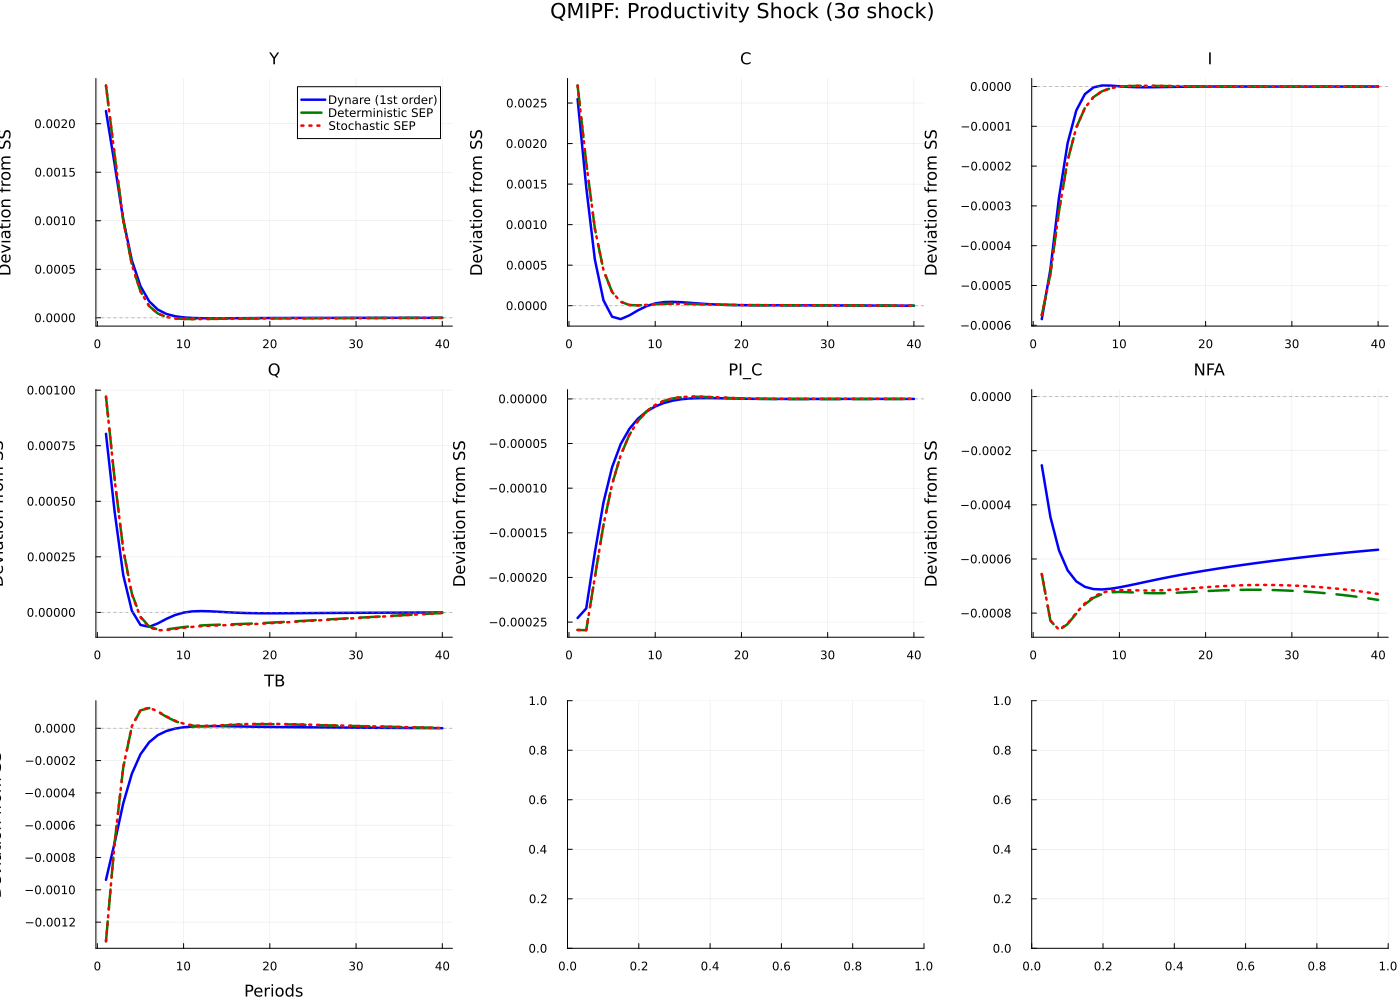
\includegraphics[width=\textwidth]{figures/QMIPF_EPS_Z_3sigma.pdf}
}{%
  \fbox{\parbox{0.9\textwidth}{\centering\vspace{1.5cm}3$\sigma$ shock\vspace{1.5cm}}}
}
\end{column}
\end{columns}

\vspace{0.3cm}
\centering
\textit{Red (stochastic) diverges from green (deterministic) as shock size increases}
\end{frame}

\begin{frame}{Foreign Interest Rate Shock: 2$\sigma$ and 3$\sigma$}
\begin{columns}
\begin{column}{0.5\textwidth}
\centering
\IfFileExists{figures/QMIPF_EPS_I_ST_2sigma.pdf}{%
  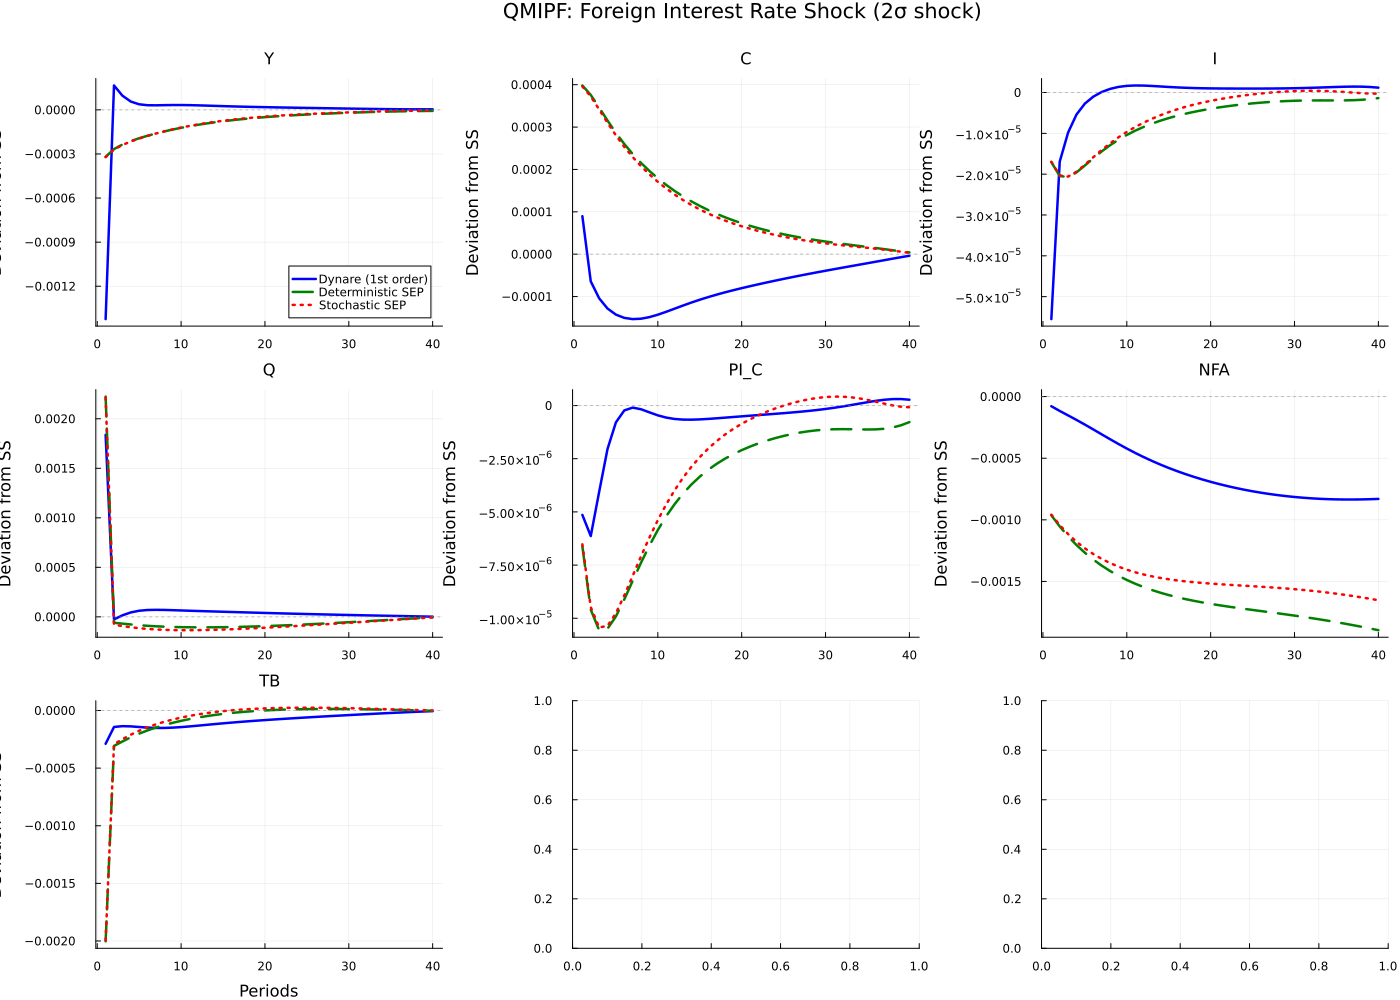
\includegraphics[width=\textwidth]{figures/QMIPF_EPS_I_ST_2sigma.pdf}
}{%
  \fbox{\parbox{0.9\textwidth}{\centering\vspace{1.5cm}2$\sigma$ shock\vspace{1.5cm}}}
}
\end{column}
\begin{column}{0.5\textwidth}
\centering
\IfFileExists{figures/QMIPF_EPS_I_ST_3sigma.pdf}{%
  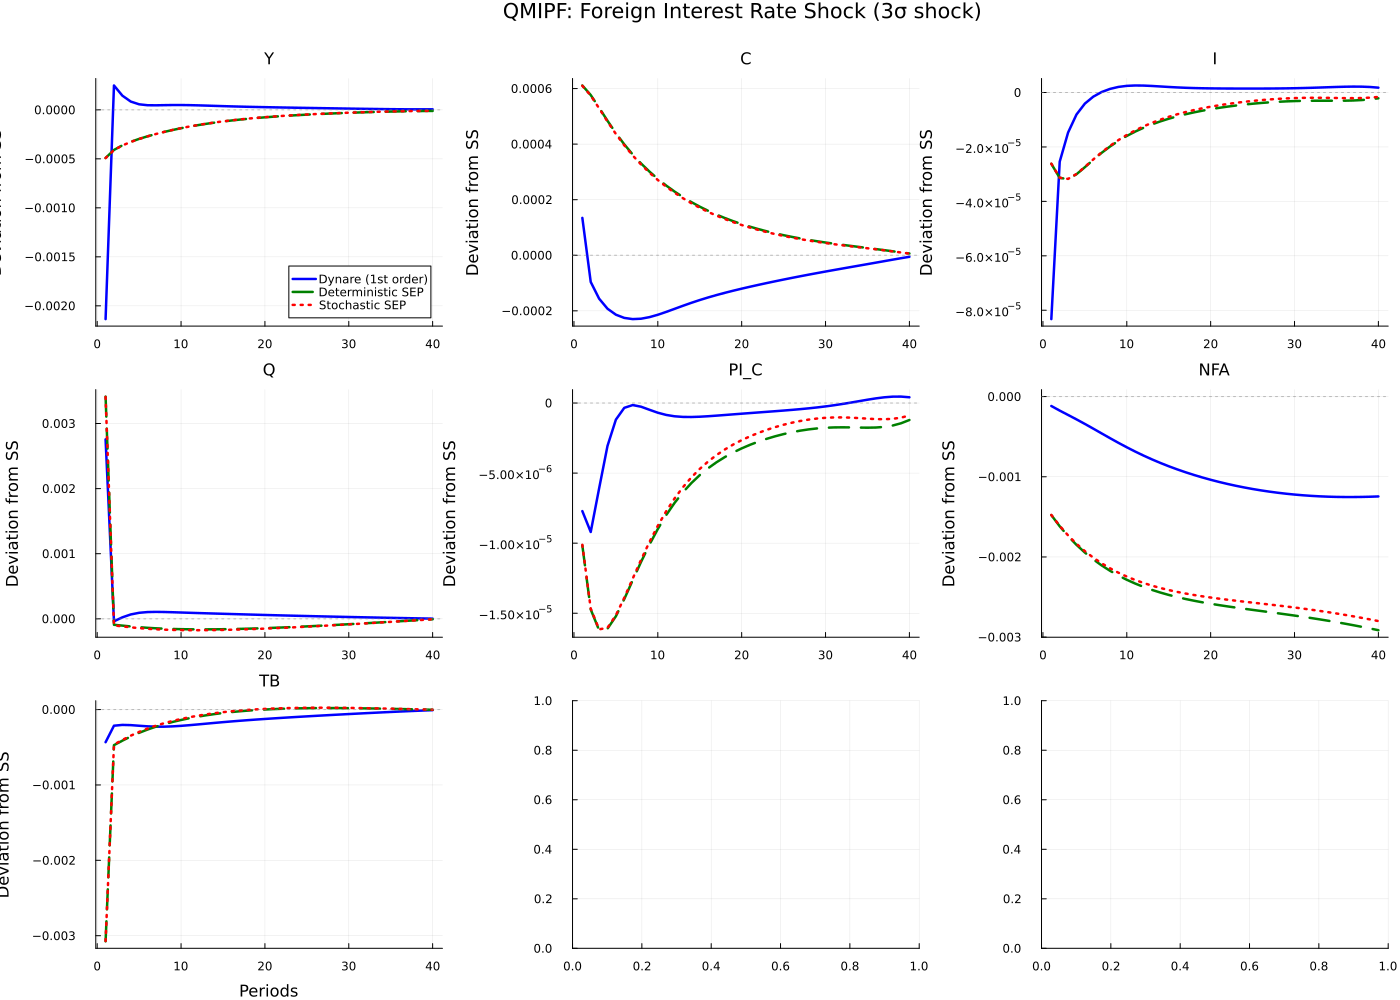
\includegraphics[width=\textwidth]{figures/QMIPF_EPS_I_ST_3sigma.pdf}
}{%
  \fbox{\parbox{0.9\textwidth}{\centering\vspace{1.5cm}3$\sigma$ shock\vspace{1.5cm}}}
}
\end{column}
\end{columns}

\vspace{0.3cm}
\centering
\textit{Capital flow dynamics show larger divergence under uncertainty}
\end{frame}

\begin{frame}{Risk Premium Shock: 2$\sigma$ and 3$\sigma$}
\begin{columns}
\begin{column}{0.5\textwidth}
\centering
\IfFileExists{figures/QMIPF_EPS_TAU_F_2sigma.pdf}{%
  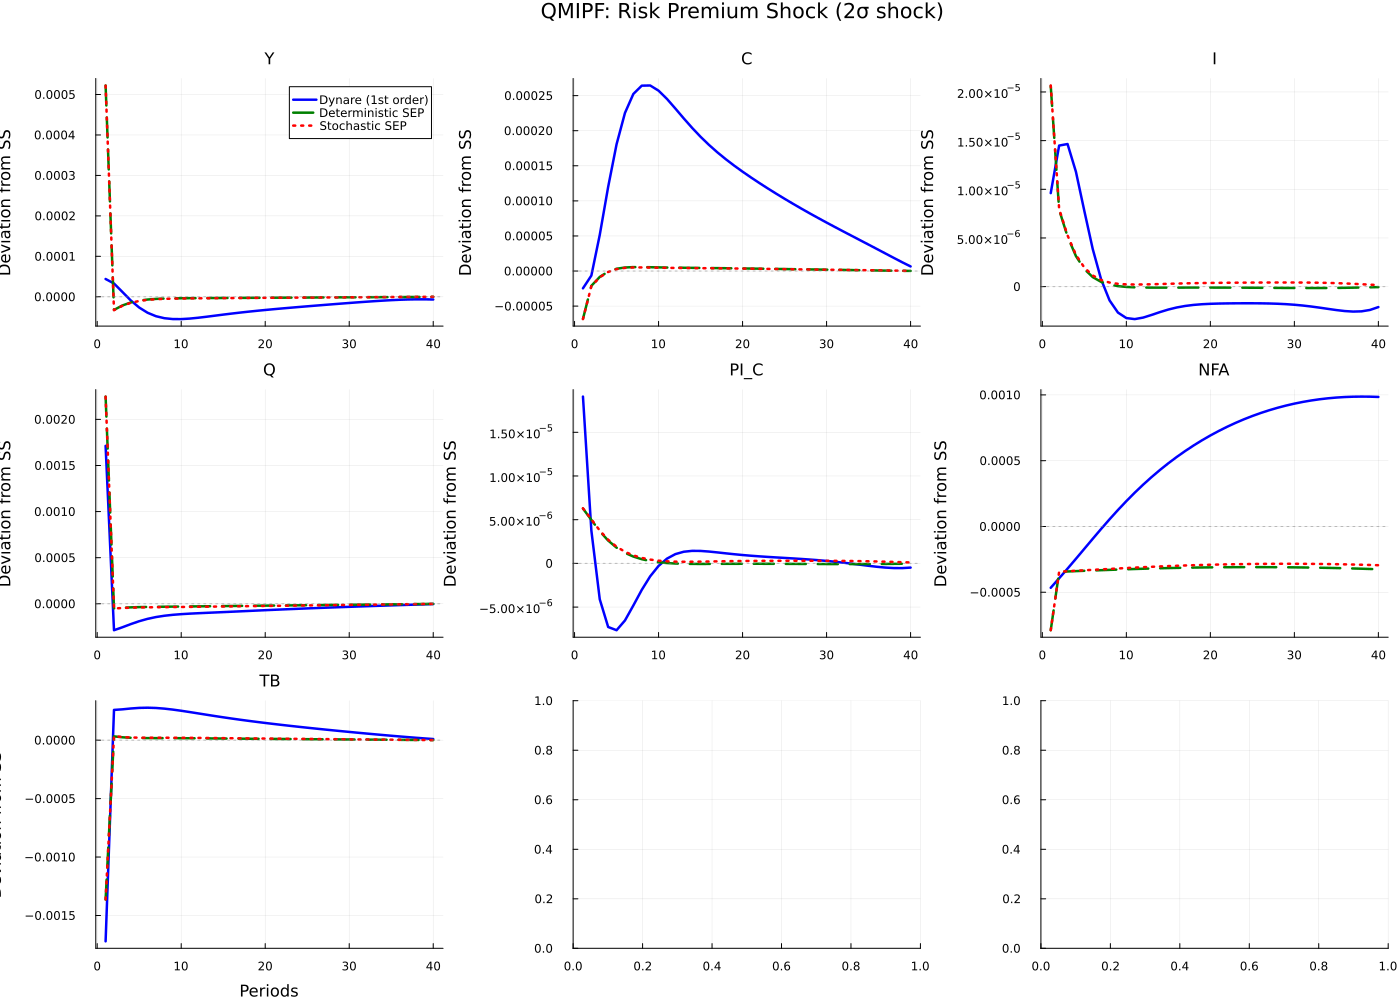
\includegraphics[width=\textwidth]{figures/QMIPF_EPS_TAU_F_2sigma.pdf}
}{%
  \fbox{\parbox{0.9\textwidth}{\centering\vspace{1.5cm}2$\sigma$ shock\vspace{1.5cm}}}
}
\end{column}
\begin{column}{0.5\textwidth}
\centering
\IfFileExists{figures/QMIPF_EPS_TAU_F_3sigma.pdf}{%
  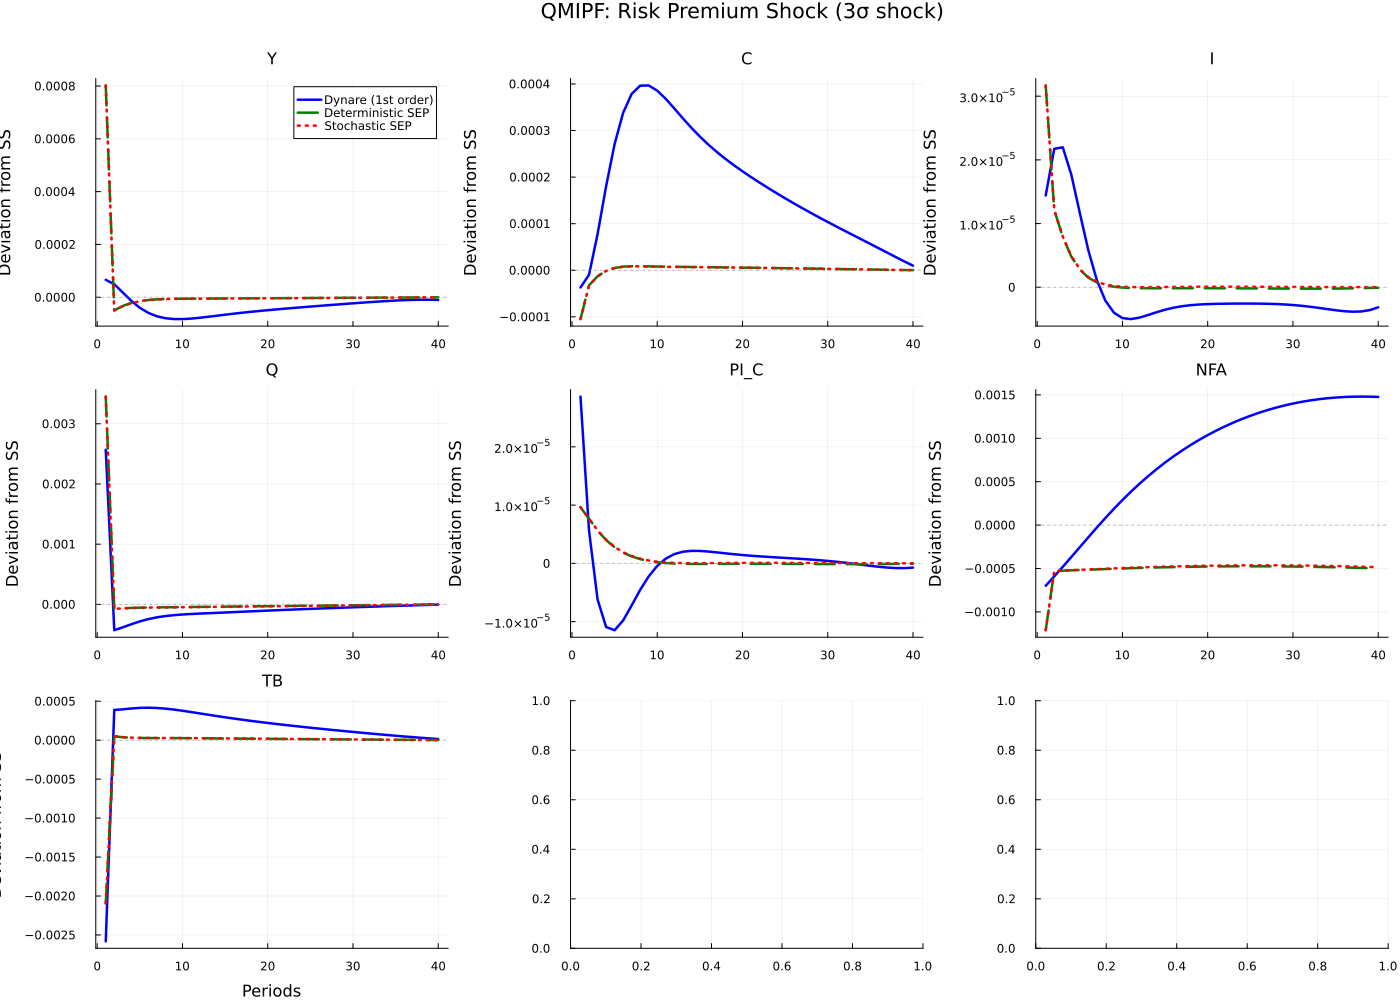
\includegraphics[width=\textwidth]{figures/QMIPF_EPS_TAU_F_3sigma.pdf}
}{%
  \fbox{\parbox{0.9\textwidth}{\centering\vspace{1.5cm}3$\sigma$ shock\vspace{1.5cm}}}
}
\end{column}
\end{columns}

\vspace{0.3cm}
\centering
\textit{FX intervention effectiveness depends on uncertainty treatment}
\end{frame}

%=============================================================================
\section{Implementation Status}
%=============================================================================

\begin{frame}{What's Working, What's Next}

\begin{columns}[T]
\begin{column}{0.5\textwidth}
\textbf{Implemented} \textcolor{green!60!black}{\checkmark}
\begin{itemize}
  \footnotesize
\item[\textcolor{green!60!black}{\checkmark}] Core QMIPF structure
\item[\textcolor{green!60!black}{\checkmark}] Calvo pricing (goods + wages)
\item[\textcolor{green!60!black}{\checkmark}] CES aggregation
\item[\textcolor{green!60!black}{\checkmark}] Real UIP + risk premium
\item[\textcolor{green!60!black}{\checkmark}] Taylor rule monetary policy
\item[\textcolor{green!60!black}{\checkmark}] SEP solver (det + stoch)
\item[\textcolor{green!60!black}{\checkmark}] MCP for constraints
\item[\textcolor{green!60!black}{\checkmark}] Full Dynare validation
\end{itemize}
\end{column}

\begin{column}{0.5\textwidth}
   \footnotesize

\textbf{Not Yet Implemented} $\square$
% \begin{itemize}
% \item[$\square$] Two-country extension
\begin{itemize}
\item Currently: foreign exogenous
% \end{itemize}
% \item[$\square$] Currency denomination of debt
% \begin{itemize}
\item Gross asset/liability positions
% \end{itemize}
% \item[$\square$] Financial intermediaries
% \begin{itemize}
\item Banking sector, leverage
% \end{itemize}
\item Bayesian estimation
% \item[$\square$] Optimal policy (Ramsey)
\end{itemize}
\end{column}
\end{columns}

\vspace{0.1cm}
\begin{block}{Computational Performance}
   \footnotesize
\begin{tabular}{ll}
Linear IRF: & $<0.1$ seconds \\
Deterministic SEP: & 2--3 seconds \\
Stochastic SEP (order=20): & 2--3 minutes per shock
\end{tabular}
\end{block}

\end{frame}

%=============================================================================
\section{Conclusions}
%=============================================================================

\begin{frame}{Bottom Line}

\begin{columns}[T]
\begin{column}{0.33\textwidth}
\begin{block}{1. Replication Successful}
\begin{itemize}
\item Julia matches Dynare
\item $<0.1\%$ difference
\item Full model structure
\end{itemize}
\end{block}
\end{column}

\begin{column}{0.33\textwidth}
\begin{block}{2. Nonlinearity Matters}
\begin{itemize}
\item 4--9\% precautionary effects
\item At 2--3$\sigma$ shocks
\item Linear understates crisis
\end{itemize}
\end{block}
\end{column}

\begin{column}{0.33\textwidth}
\begin{block}{3. Ready for Policy}
\begin{itemize}
\item SEP: scenario analysis
\item MCP: ZLB, debt limits
\item Transparent, shareable
\end{itemize}
\end{block}
\end{column}
\end{columns}

\vspace{0.5cm}
\textbf{Next Steps}
\begin{itemize}
\item Two-country extension for spillover analysis
\item Estimation on EME data
\item Optimal policy under uncertainty
\end{itemize}

\vspace{0.3cm}
\centering
\textbf{Code available:} \texttt{MacroModelling\_local/models/QMIPF\_final.jl}

\end{frame}

%=============================================================================
% Backup slides
%=============================================================================

\appendix

\begin{frame}{Backup: Quantitative Results}

\begin{table}
\centering
\small
\begin{tabular}{lrrr}
\toprule
\textbf{Variable} & \textbf{Deterministic} & \textbf{Stochastic} & \textbf{$\Delta$} \\
\midrule
\multicolumn{4}{l}{\textit{Foreign Interest Rate Shock}} \\
$Y$ & 0.002351 & 0.002238 & $-4.8\%$ \\
$C$ & 0.002698 & 0.002601 & $-3.6\%$ \\
$I$ & 0.000215 & 0.000198 & $-7.9\%$ \\
$Q$ & 0.010210 & 0.009849 & $-3.5\%$ \\
$\Pi^C$ & 0.000120 & 0.000109 & $-9.2\%$ \\
$NFA$ & 0.022093 & 0.022228 & $+0.6\%$ \\
$TB$ & 0.013927 & 0.013402 & $-3.8\%$ \\
\bottomrule
\end{tabular}
\caption{Peak responses: Deterministic vs Stochastic SEP}
\end{table}

\end{frame}

\begin{frame}{Backup: SEP Algorithm}

\textbf{Stochastic Extended Path} \citep{adjemian2025stochastic}

\begin{enumerate}
\item Start from initial state $x_0$
\item For each period $t = 1, \ldots, T$:
\begin{itemize}
\item Construct quadrature nodes for future shocks
\item Solve nonlinear system at each node
\item Weight by Gauss-Hermite probabilities
\item Aggregate to get expected path
\end{itemize}
\item Iterate until convergence ($\|x^{(k+1)} - x^{(k)}\| < \epsilon$)
\end{enumerate}

\vspace{0.3cm}
\textbf{Parameters Used}
\begin{itemize}
\item Order = 20 (look-ahead periods)
\item Nodes = 3 (per shock dimension)
\item Tolerance = $5 \times 10^{-5}$
\item Max iterations = 2000
\item Sparse tree = true (computational efficiency)
\end{itemize}

\end{frame}

\begin{frame}[allowframebreaks]{References}
\small
\begin{thebibliography}{99}

\bibitem[Adrian et al., 2020]{adrian2020conceptual}
Adrian, T., et al. (2020).
\newblock A Quantitative Model for the Integrated Policy Framework.
\newblock \textit{IMF Working Paper} 20/122.

\bibitem[Adrian et al., 2021]{adrian2021quantitative}
Adrian, T., et al. (2021).
\newblock The Quantitative Microfounded Model for the Integrated Policy Framework.
\newblock \textit{IMF Working Paper} 21/292.

\bibitem[Adjemian \& Julliard, 2025]{adjemian2025stochastic}
Adjemian, S. \& Julliard, M. (2025).
\newblock Stochastic Extended Path.
\newblock \textit{Dynare Working Papers} 84, CEPREMAP.

\end{thebibliography}
\end{frame}

\end{document}
